% !TEX encoding = UTF-8 Unicode
\chapter{Konzepte}
Die Konzepte welche Esper verwendet werdet, dienen dazu, den kompletten Ereignisfluss von der Aktion bis zur Verarbeitung und nachfolgenden Aktionen, abzubilden.
Ereignisse werden dezentral gefeuert und sind, durch die Registrierung der Ereignistypen auf dem Ereignis-Prozessor, klar definiert. Je nach hinterlegtem Regelwerk, werden diese, von einer Event-Engine, erfasst und verarbeitet oder ignoriert. Zur Regeldefinition dienen Muster, welche als Statements umgesetzt werden. Die Ereignismuster können verschiedene Techniken verwenden, nach denen der Ereignisstrom untersucht wird. Im folgenden werden die eben erwähnten Komponenten näher erläutert.

\section{Statements}

Statements dienen dazu Muster zu definieren, mit deren Hilfe die Event-Engine den Datenstrom analysiert. Hierzu existiert die \acf{EPL}, welche stark an den Syntax von SQL erinnert. Mit ihrer Hilfe wird die Ereignisverarbeitung in Esper umgesetzt.

\section{Select}

Quelltext \ref{basic_select} zeigt ein einfaches Select-Statement. Resultierend hieraus, wird der \acf{EP} auf alle Ereignisse vom Typ \textit{Action} reagieren und diese bei Eintritt erfassen. Sie werden unverändert weitergegeben. Dieses Statement wird im dem Casino eingesetzt, um über sämtliche Züge informiert zu werden. Erkennbar ist jedoch nicht, welcher Zug zu welchem Spiel, etc. gehört. Um Ereignisse feingranular untersuchen zu können, werden weitere Techniken benötigt, welche beispielsweise nach Attributen filtern können.

\begin{lstlisting}[caption={Statement Selektion}\label{basic_select},captionpos=b,language=SQL]

select * from GameActionEvent

\end{lstlisting}

\begin{figure}[h]
	\centering
	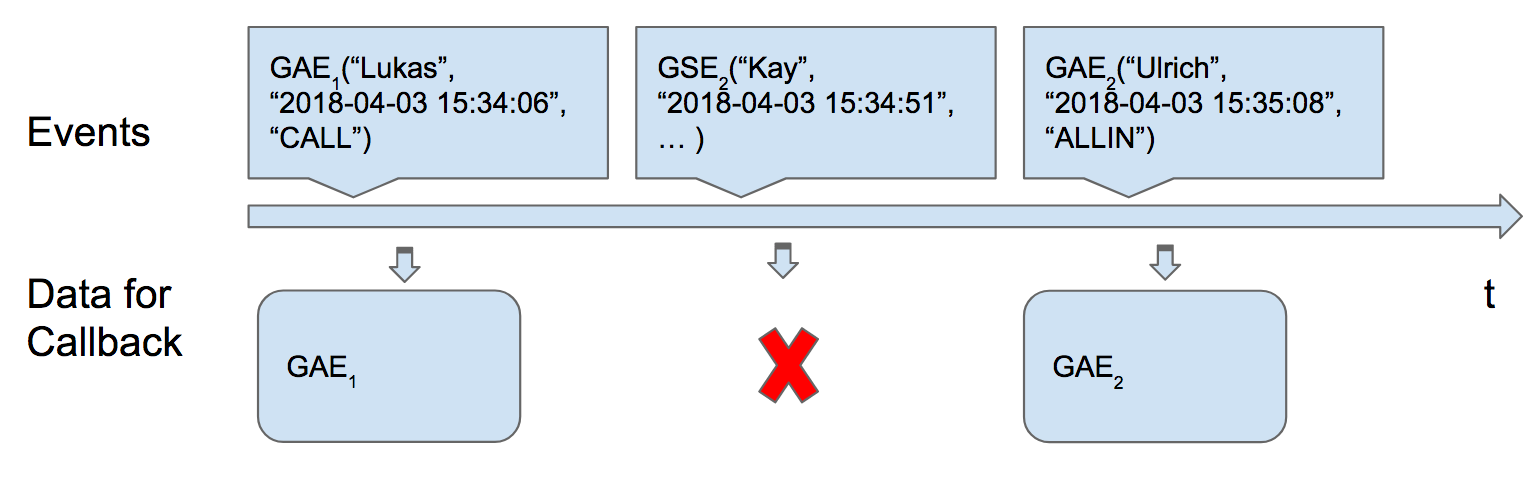
\includegraphics[width=\textwidth,height=\textheight, keepaspectratio]{images/statement_basic_select.png}
	\caption{Ablauf Quelltext 1}
	\label{basic_select}
\end{figure}

\section{Filter}

Die Filterfunktion ist eine geeignete Möglichkeit, die Selektion aus dem Ereignisfluss auf definierte Attribute zu beschränken. Wie das Beispiel in Quelltext \ref{filter_select} veranschaulicht, können, wie im SQL Syntax, Ereigniseigenschaften beschränkt werden.
Es werden nur die Attribute \textit{playerName} und \textit{deck} der auftretenden Ereignisse vom Typ \textit{GameEnd} berücksichtigt und weiterverarbeitet, wie Abbildung (\ref{filter_select}) zeigt.
Das Casino benötigt ein solches Statement, um zu erfahren, wer welches Spiel mit welcher Hand gewonnen wird. Um jedoch, einen Spieler mit oftmaligem Glück zu entdecken, ist die Anzahl der Siege erwünscht. Hierfür können die selektierten Daten, mit weiteren Funktionen aggregiert werden.

\begin{lstlisting}[caption={Statement mit Filter}\label{filter_select},captionpos=b,language=SQL]

select playerName, deck from GameEndEvent

\end{lstlisting}

\begin{figure}[ht]
	\centering
	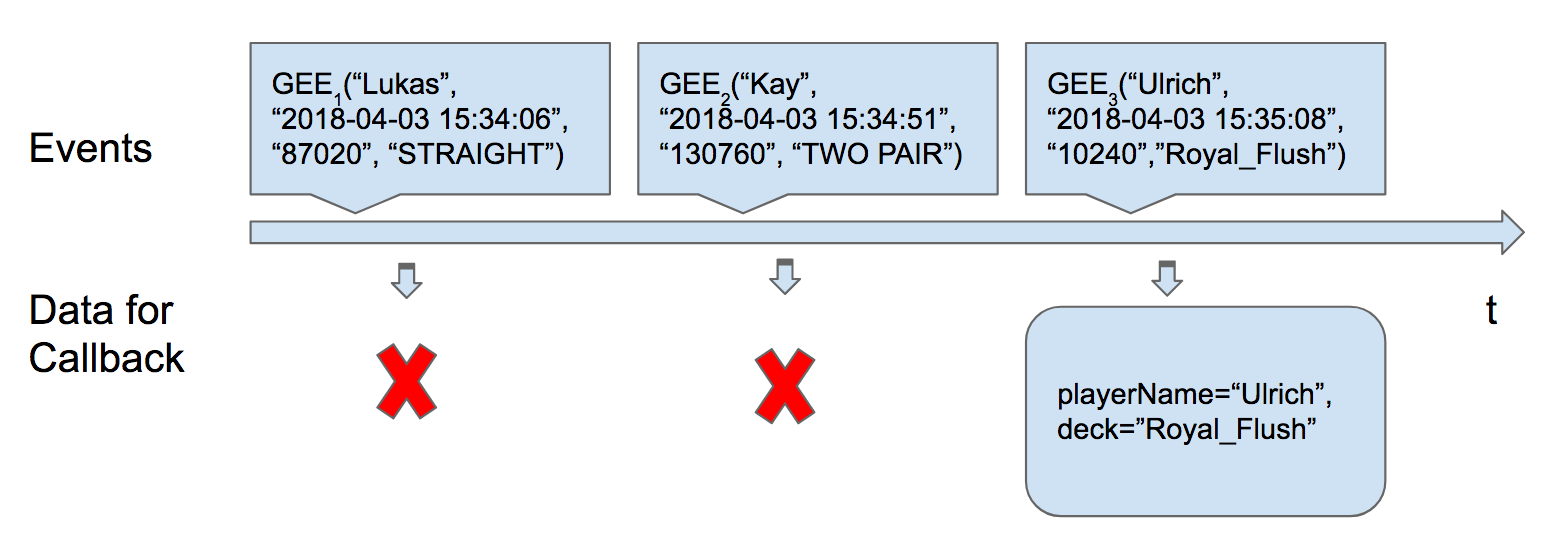
\includegraphics[width=\textwidth,height=\textheight, keepaspectratio]{images/statement_basic_filter.png}
	\caption{Ablauf Quelltext 2}
	\label{filter_select}
\end{figure}

\section{Aggregation}

Um zu erfahren, welcher Spieler wie oft gewonnen hat wird die Aggregationsfunktion \textit{count(playerName)}. Quelltext \ref{aggregation_select} zeigt das dazu passende Statement. Dies hat zur Folge, dass der Ereignisstrom die auftretenden Ereignisse vom Typ \textit{GameEvent} mit selbem Spieler-Namen zählt. Der errechnete Wert wird mithilfe von \textit{as wins} in eine neues Attribut mit Alias "wins" gespeichert. Weitere Aggregationsfunktionen wie \textit{sum()}, \textit{avg()}, usw. sind ebenso verfügbar.
Im Casino fällt auf, dass sich die Spielenden der Vortage in den zu analysierenden Daten befinden. Um nur die Daten des aktuellen Tages auswerten zu können, sind Beschränkungen des auszuwertenden Ereignisstroms erforderlich. Die \acf{EPL} bietet hierfür sogenannte Data-Windows.

\begin{lstlisting}[caption={Statement mit Aggregation}\label{aggregation_select},captionpos=b,language=SQL]

select playerName, count(playerName) as wins, deck from GameEndEvent

\end{lstlisting}

\section{Data-Windows}
\label{Data-Windows}

\section{Patterns}

Eine Alternative zu den Select-Satements stellen Abfragen nach Strukturen, sogenannte Patterns dar. Events, welche den Bedingungen entsprechen werden erfasst. Hierbei kommen verschiedene Elemente bei der Pattern-Definition zum Einsatz.

\begin{enumerate}
	\item Kontrolloperator: \texttt{every} definiert die Erstellung eines Pattern und regelt die Abarbeitung. Es wird alle(eng. every) auf das Ereignismuster zutreffende Ereignisse erfasst. Ein simples Pattern, welches alle Ereignisse des eines Tages vom Typ \textit{GameActionEvent} erfasst, kann Quellcode \ref{basic_pattern} entnommen werden.
	In der \texttt{where}-Klausel können weitere Bedingungen, ähnlich wie bei der Selektion, definiert werden.
	
	\begin{lstlisting}[caption={Einfaches Pattern mit Where-Klausel}\label{basic_pattern}, captionpos=b,language=SQL]
	
	every GameActionEvent where timer:within(28800 seconds)
	
	\end{lstlisting}
	
	\item Logische Operatoren: 
	Das Pattern kann, wie in Quellcode \ref{logic_pattern} veranschaulicht, durch logische Operatoren wie \texttt{and, or , not} zusammengesetzt werden. So kann wie in Quellcode \ref{logic_pattern} das Ereignismuster mit Bedingungen bestückt werden. In diesem Beispiel würden Events vom Typ \textit{GameEnd} oder vom Typ \textit{GameAction} erfasst werden.
	
	\begin{lstlisting}[caption={Pattern mit logischen Operatoren}\label{logic_pattern},captionpos=b,language=SQL]
	
	every a=GameActionEvent or b=GameActionEvent
	
	\end{lstlisting}
	
	\item Nachfolge-Operator:
	Der Nachfolge-Operator \texttt{->} tritt ein wenn das davor, gefolgt vom danach definiertem Ereignis eintrifft. In Quellcode \ref{follow_pattern}  würden alle Endevents betrachtet, welche auf ein Aktionsevent folgen. Die Bedingung trifft zu, wenn der vorangegangene Zug ein Spielausstieg(\textit{action = "FOLD"}) war.
	Wie im Quellcode zu erkennen ist, werden die Ereignisse in Variablen \textit{a, b} gespeichert(bspw. \textit{a=GameAction}). So können die Werte im nächsten Schritt weiterverwendet werden. Im Beispiel wird das Folgeevent (\textit{b=GameEnd(a.playerName != b.playerName)}) überprüfen ob der Spieler-Name ungleich dem vorherigen ist und im Erfolgsfall erfasst. Auf diese Art und Weise lassen ich komplexe bedingte Ereignismuster definieren.
	
	\begin{lstlisting}[caption={Pattern mit Follow-Operator }\label{follow_pattern},captionpos=b,language=SQL]
	
	every a = GameActionEvent(action="FOLD") -> b =
	 GameEndEvent(a.playerName != b.playerName)
	
	\end{lstlisting}
	
	\item Zeitliche Beobachter (engl. Observer):
	Das letzte, wie zum Beispiel Zeit-Überwacher, können nach der \texttt{where}-Klausel angegeben werden. Beispielsweise kann ein Timer, welcher den Ereignisstrom beschränkt, mit \texttt{timer:within} definiert werden. Dieser kann mit \texttt{timer:interval}
	\texttt{timer:at}
	...
\end{enumerate}


\section{Partitions}

\section{Kombinierte Statements}

